\documentclass[final,t]{beamer}\usepackage[]{graphicx}\usepackage[]{color}
%% maxwidth is the original width if it is less than linewidth
%% otherwise use linewidth (to make sure the graphics do not exceed the margin)
\makeatletter
\def\maxwidth{ %
  \ifdim\Gin@nat@width>\linewidth
    \linewidth
  \else
    \Gin@nat@width
  \fi
}
\makeatother

\definecolor{fgcolor}{rgb}{0.345, 0.345, 0.345}
\newcommand{\hlnum}[1]{\textcolor[rgb]{0.686,0.059,0.569}{#1}}%
\newcommand{\hlstr}[1]{\textcolor[rgb]{0.192,0.494,0.8}{#1}}%
\newcommand{\hlcom}[1]{\textcolor[rgb]{0.678,0.584,0.686}{\textit{#1}}}%
\newcommand{\hlopt}[1]{\textcolor[rgb]{0,0,0}{#1}}%
\newcommand{\hlstd}[1]{\textcolor[rgb]{0.345,0.345,0.345}{#1}}%
\newcommand{\hlkwa}[1]{\textcolor[rgb]{0.161,0.373,0.58}{\textbf{#1}}}%
\newcommand{\hlkwb}[1]{\textcolor[rgb]{0.69,0.353,0.396}{#1}}%
\newcommand{\hlkwc}[1]{\textcolor[rgb]{0.333,0.667,0.333}{#1}}%
\newcommand{\hlkwd}[1]{\textcolor[rgb]{0.737,0.353,0.396}{\textbf{#1}}}%

\usepackage{framed}
\makeatletter
\newenvironment{kframe}{%
 \def\at@end@of@kframe{}%
 \ifinner\ifhmode%
  \def\at@end@of@kframe{\end{minipage}}%
  \begin{minipage}{\columnwidth}%
 \fi\fi%
 \def\FrameCommand##1{\hskip\@totalleftmargin \hskip-\fboxsep
 \colorbox{shadecolor}{##1}\hskip-\fboxsep
     % There is no \\@totalrightmargin, so:
     \hskip-\linewidth \hskip-\@totalleftmargin \hskip\columnwidth}%
 \MakeFramed {\advance\hsize-\width
   \@totalleftmargin\z@ \linewidth\hsize
   \@setminipage}}%
 {\par\unskip\endMakeFramed%
 \at@end@of@kframe}
\makeatother

\definecolor{shadecolor}{rgb}{.97, .97, .97}
\definecolor{messagecolor}{rgb}{0, 0, 0}
\definecolor{warningcolor}{rgb}{1, 0, 1}
\definecolor{errorcolor}{rgb}{1, 0, 0}
\newenvironment{knitrout}{}{} % an empty environment to be redefined in TeX

\usepackage{alltt}




%% Examples:
%% http://www-i6.informatik.rwth-aachen.de/~dreuw/latexbeamerposter.php
\mode<presentation> {
  %% TODO(chogg): define my own theme
  %% (e.g. for big headlines using my own logos)
  \usetheme{I6pd2}
}
\usepackage[english]{babel}
\usepackage[latin1]{inputenc}
\usepackage{amsmath,amsthm,amssymb,latexsym}
\usepackage{pifont}
\newcommand{\cmark}{\ding{51}}%
\newcommand{\xmark}{\ding{55}}%
\usefonttheme[onlymath]{serif}
\boldmath
\usepackage[orientation=landscape,size=a0,scale=1.4,debug]{beamerposter}                       % e.g. for DIN-A0 poster
\title[Smooth Animations]{\huge Smooth Animations to Visualize Gaussian Uncertainty}
\author{Charles~R.~Hogg~III}
\institute[Google]{Google, Inc.}
\date{July 16, 2014}
\IfFileExists{upquote.sty}{\usepackage{upquote}}{}
\begin{document}
\begin{frame}[fragile]
  \begin{columns}[T,onlytextwidth]

    % Left column.
    \begin{column}{.32\linewidth}

      \begin{block}{Introduction}
        \begin{itemize}
          \item \textbf{Goal:} Visualize uncertainty in \textit{curves and
            surfaces}
          \item \textbf{Approach:} animations
            \begin{itemize}
              \item Each frame shows one draw from posterior
              \item Consecutive frames differ infinitesimally (i.e.,
                \textit{continuous} animations)
            \end{itemize}
          \item \textbf{Results:}
            \begin{itemize}
              \item \textbf{Smooth, keyframe-free} animations (moving
                \textit{beyond interpolation})
              \item \textbf{New framework} for all future work in Gaussian
                animations
            \end{itemize}
        \end{itemize}
      \end{block}

      \begin{block}{Interpolation caveats}
\begin{knitrout}
\definecolor{shadecolor}{rgb}{0.969, 0.969, 0.969}\color{fgcolor}
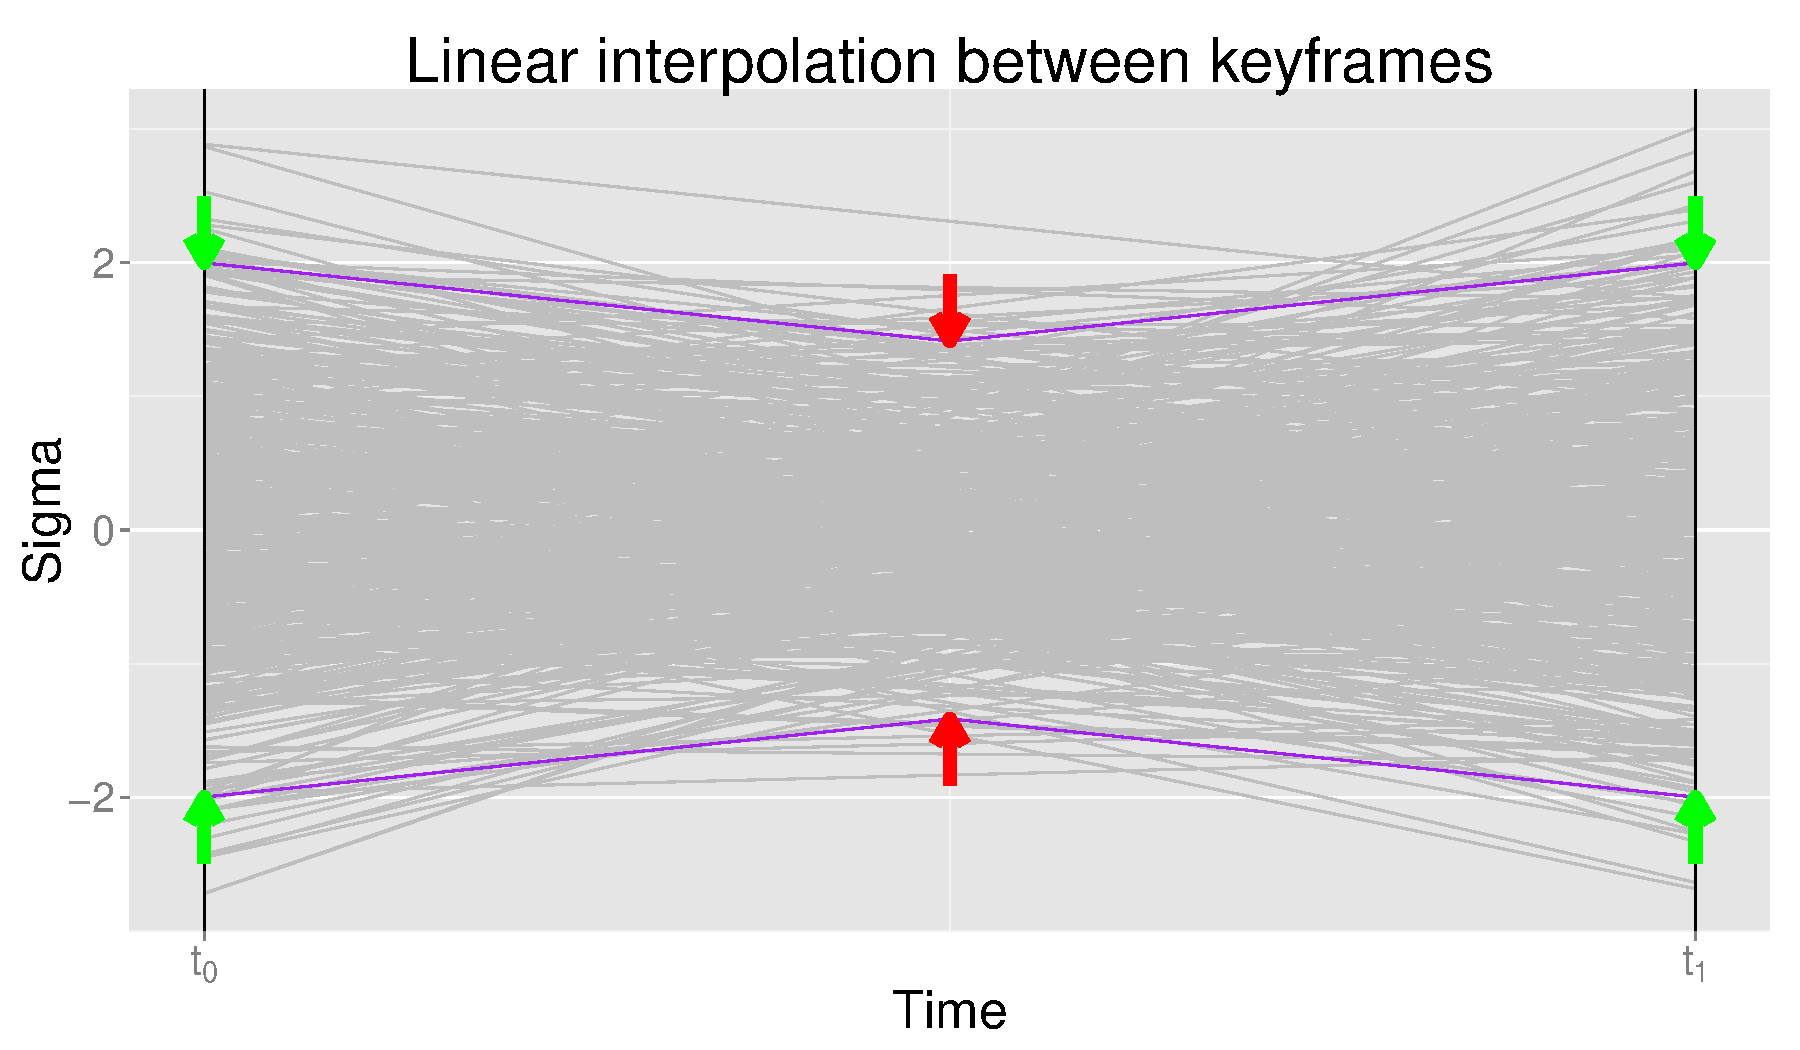
\includegraphics[width=\maxwidth]{figure/interpolation} 

\end{knitrout}

        Na\"{i}ve interpolation: \textbf{variance too small} between keyframes
        \\ \huge Next up: make side-by-side figure with ESG.  Show \textbf{actual}
        quantiles.  (Means I need to make x-values and interpolate...)
      \end{block}

    \end{column}

    % Middle column.
    \begin{column}{.32\linewidth}

      \begin{block}{Basis function view}


        \begin{table}
          \begin{tabular}{|l|c|c|c|}
            \hline
            Animation Method
            & \parbox[t][2.5em]{5em}{Statistically \\ Correct}
            & Stationary
            & Smooth \\
            \hline
\begin{knitrout}
\definecolor{shadecolor}{rgb}{0.969, 0.969, 0.969}\color{fgcolor}
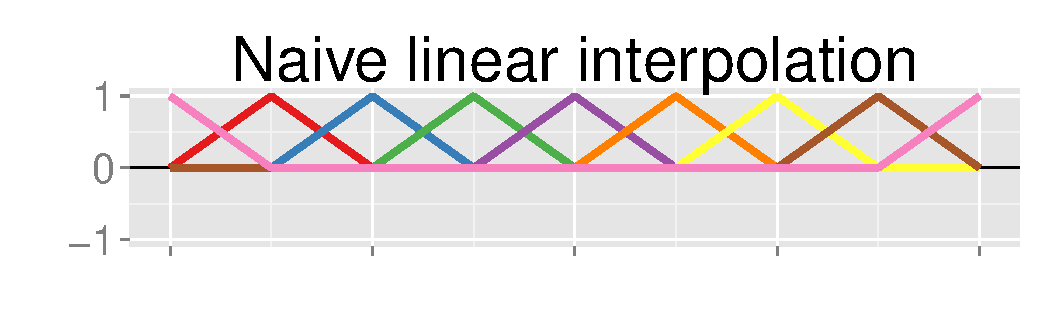
\includegraphics[width=\maxwidth]{figure/basis_linear} 

\end{knitrout}

            & {\Huge \color{red}{\xmark}} & {\Huge \color{red}{\xmark}} &
            {\Huge \color{red}{\xmark}} \\
            \hline
\begin{knitrout}
\definecolor{shadecolor}{rgb}{0.969, 0.969, 0.969}\color{fgcolor}
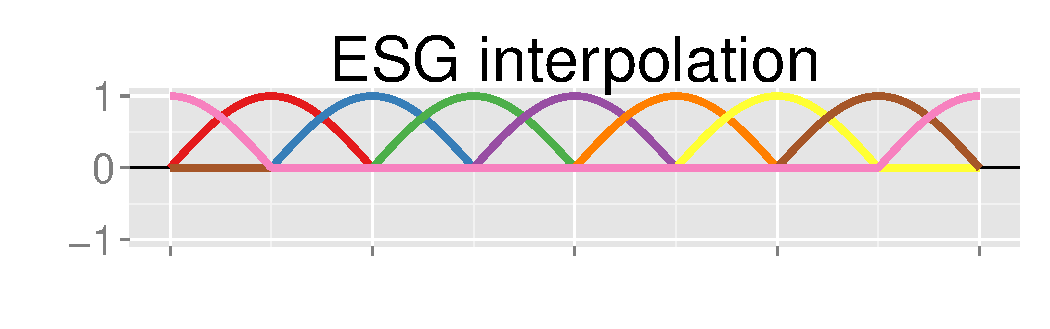
\includegraphics[width=\maxwidth]{figure/basis_esg} 

\end{knitrout}

            & {\Huge \color{green}{\cmark}} & {\Huge \color{red}{\xmark}} &
            {\Huge \color{red}{\xmark}} \\
            \hline
\begin{knitrout}
\definecolor{shadecolor}{rgb}{0.969, 0.969, 0.969}\color{fgcolor}
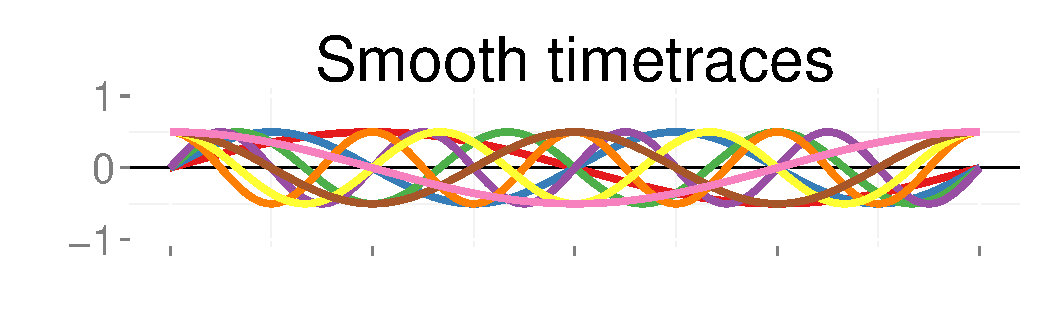
\includegraphics[width=\maxwidth]{figure/basis_smooth} 

\end{knitrout}

            & {\Huge \color{green}{\cmark}} & {\Huge \color{green}{\cmark}} &
            {\Huge \color{green}{\cmark}} \\
            \hline
          \end{tabular}
        \end{table}

      \end{block}

      \begin{block}{Physical motion: basic kinematics}
        {\small Check \textit{velocity} and \textit{acceleration} for a
        fuller picture of how these animations move:} \\
\begin{knitrout}
\definecolor{shadecolor}{rgb}{0.969, 0.969, 0.969}\color{fgcolor}
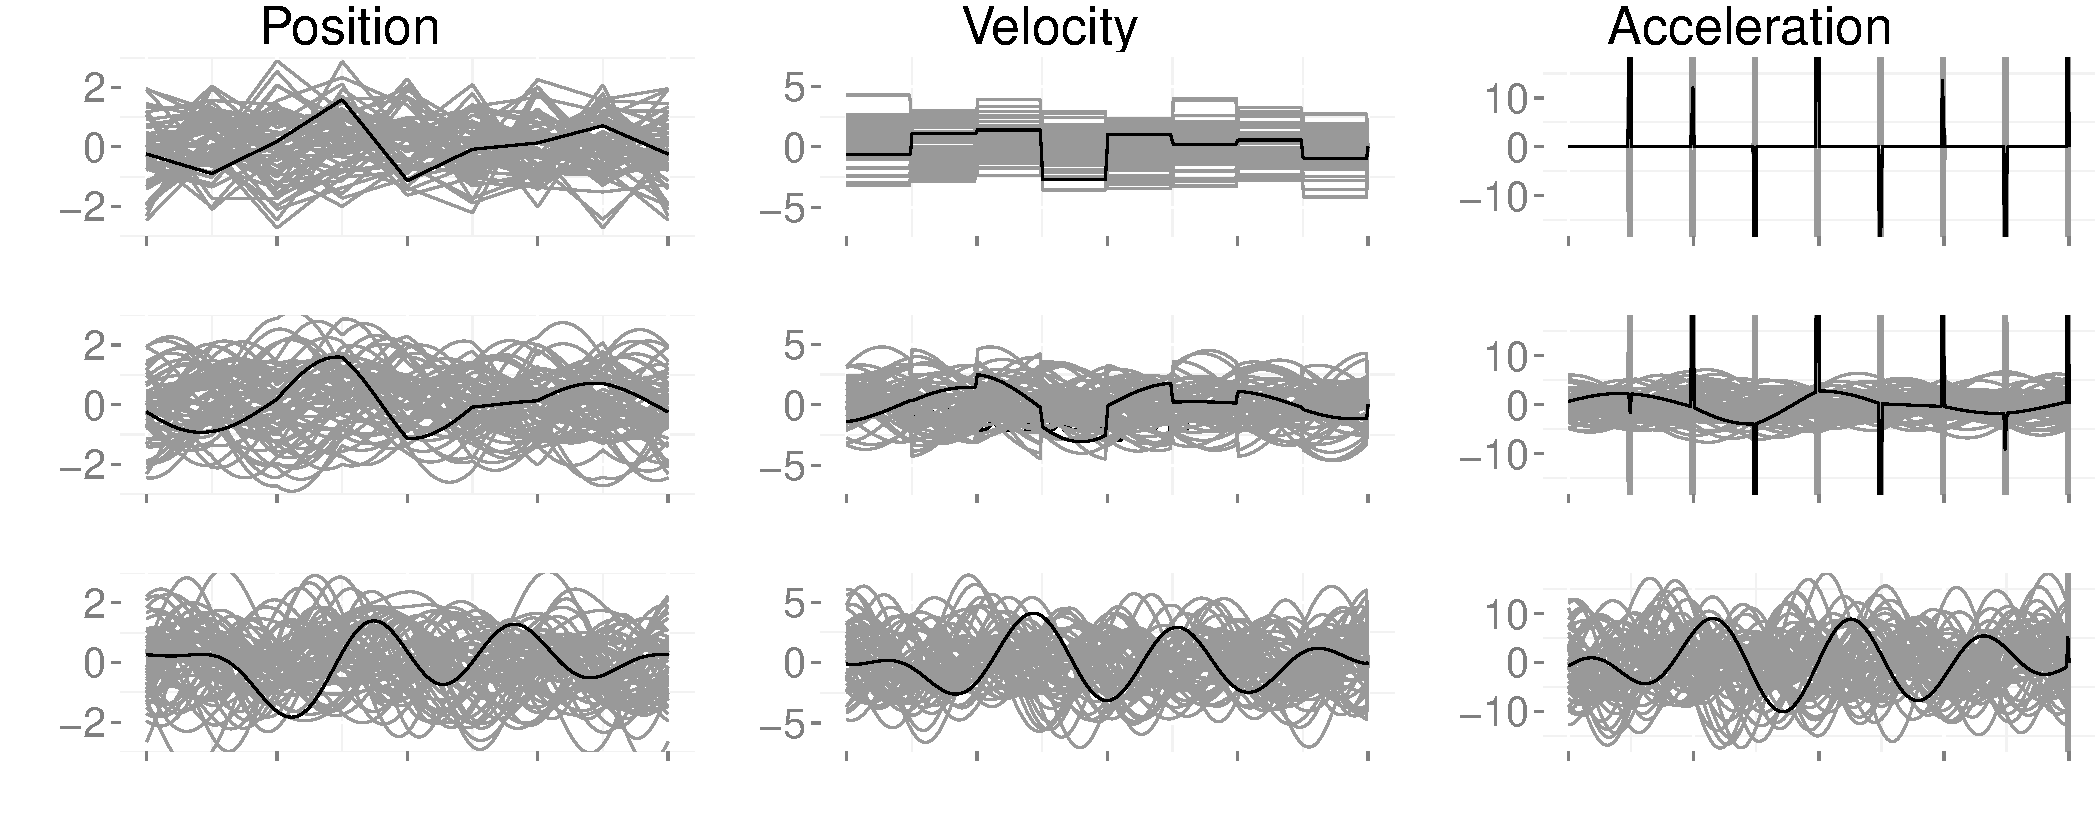
\includegraphics[width=\maxwidth]{figure/kinematics} 

\end{knitrout}

        Motion is \textit{not different} at the keyframes
        \textbf{because they do not exist.}
        \\ \tiny (Also: add the dots, in the plots!)
      \end{block}

    \end{column}

    % Right column.
    \begin{column}{.32\linewidth}

      \begin{block}{The Infinite Limit}
      \end{block}

      \begin{block}{Conclusion}
      \end{block}

    \end{column}

  \end{columns}

  \begin{block}{Gaussian Processes refresher: Probabilities for Functions}
    \begin{columns}[T]
      \begin{column}{0.16\linewidth}
        \begin{itemize}
          \item Random curves and surfaces: \\
            \textit{infinitely many} random variables!
          \item \textbf{Gaussian Processes:} \\
            work with \textit{any \textbf{finite} subset}
            \begin{itemize}
              \item Assume \textit{joint Gaussian distribution}
            \end{itemize}
          \item Simple example: \\
            Start with 2 variables, \\
            work up from there...
        \end{itemize}
      \end{column}
      \begin{column}{0.12\linewidth}
\begin{knitrout}
\definecolor{shadecolor}{rgb}{0.969, 0.969, 0.969}\color{fgcolor}
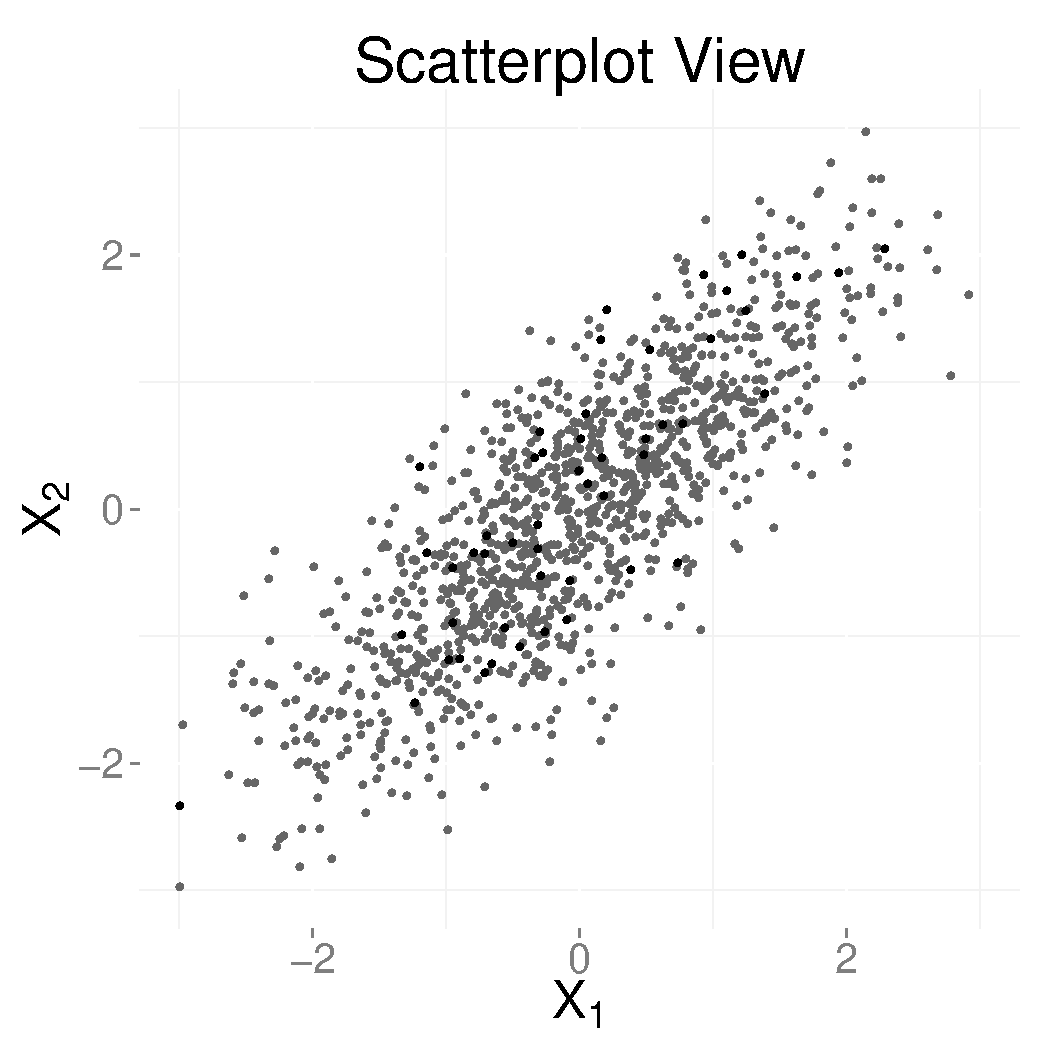
\includegraphics[width=\maxwidth]{figure/scatterplot_function} 

\end{knitrout}

        \tiny
        \begin{itemize} \scriptsize
          \item Highly correlated $\rightarrow$ \textbf{close to diagonal}
          \item Works well for two variables
        \end{itemize}
      \end{column}
      \begin{column}{0.12\linewidth}
\begin{knitrout}
\definecolor{shadecolor}{rgb}{0.969, 0.969, 0.969}\color{fgcolor}
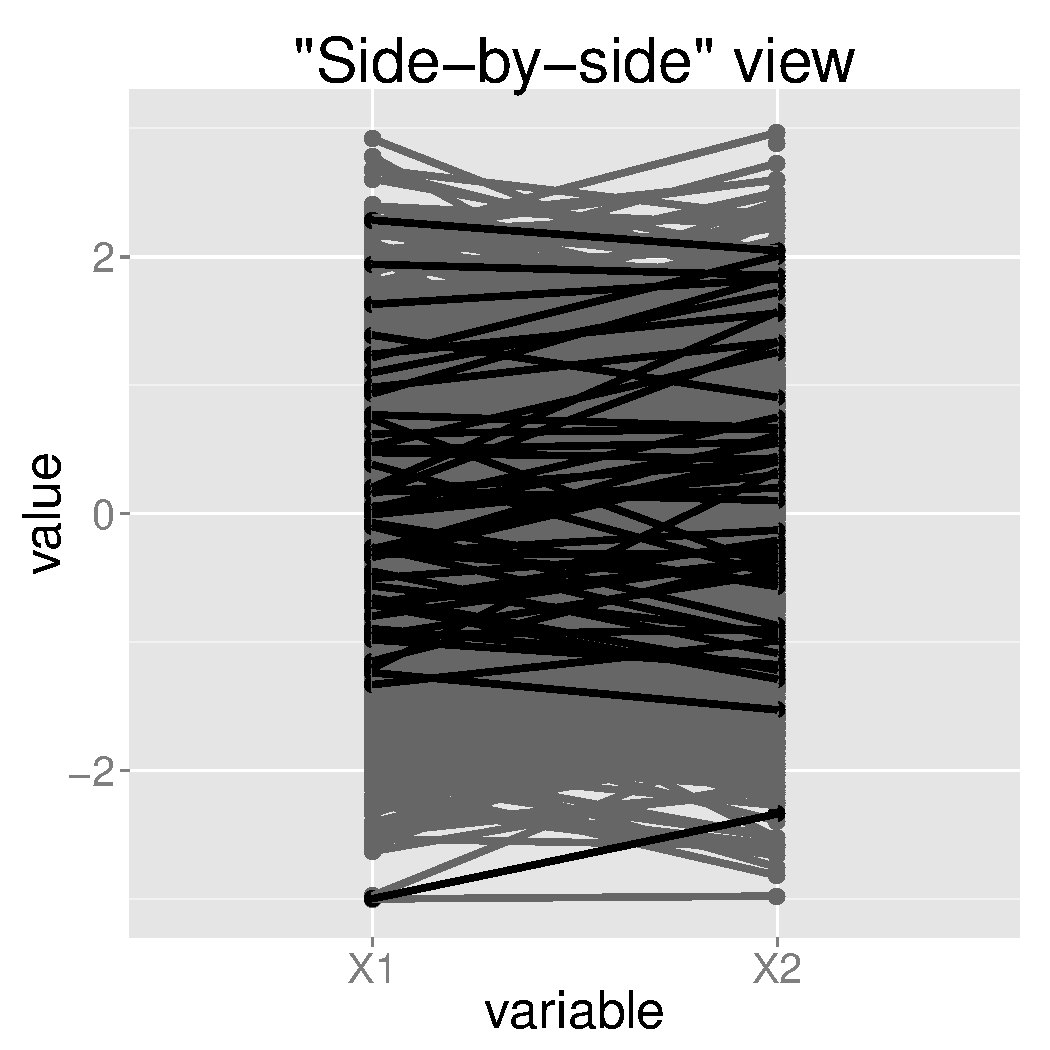
\includegraphics[width=\maxwidth]{figure/side_by_side} 

\end{knitrout}

        \begin{itemize} \scriptsize
          \item Highly correlated $\rightarrow$ \textbf{horizontal lines}
          \item Works well for more variables...
        \end{itemize}
      \end{column}
      \begin{column}{0.12\linewidth}
\begin{knitrout}
\definecolor{shadecolor}{rgb}{0.969, 0.969, 0.969}\color{fgcolor}
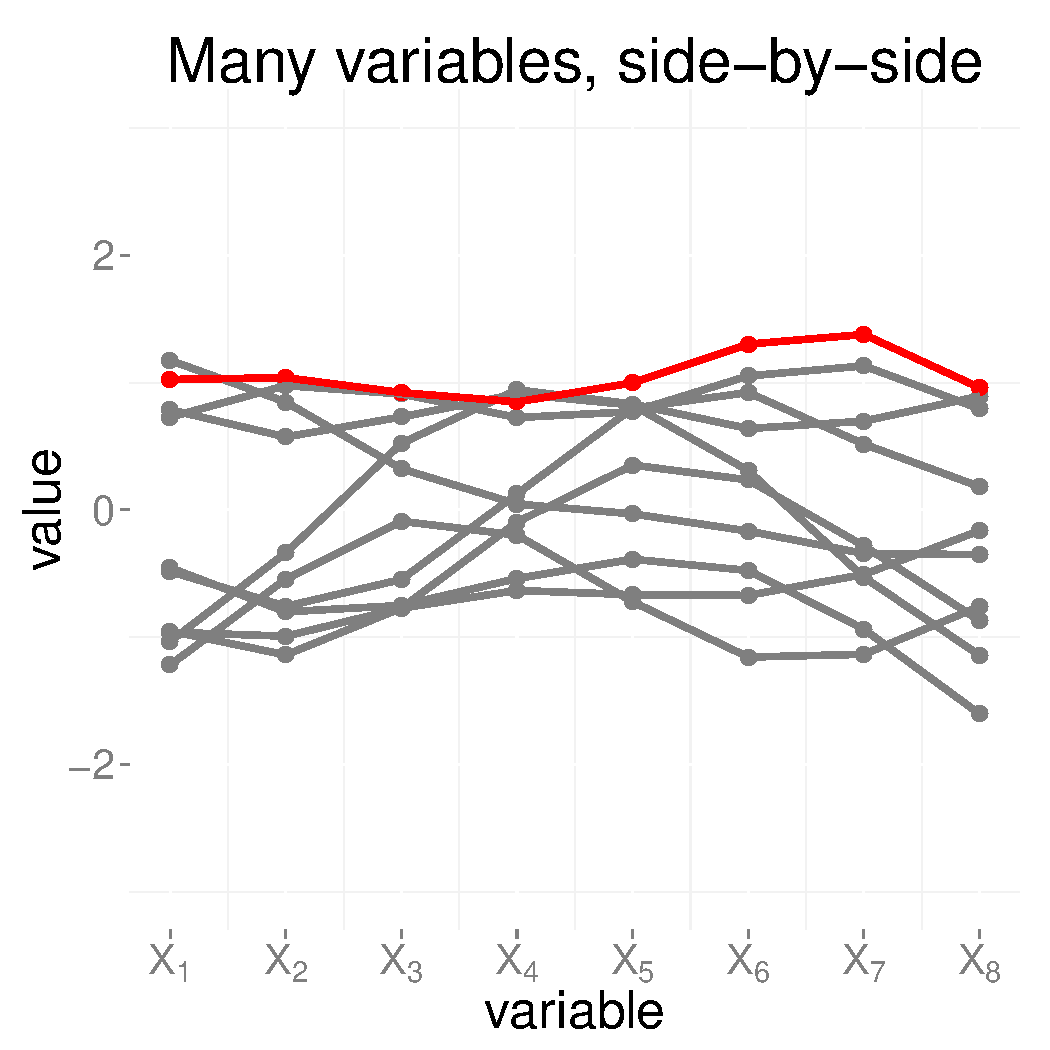
\includegraphics[width=\maxwidth]{figure/many_side_by_side} 

\end{knitrout}

        \begin{itemize} \scriptsize
          \item Variables indexed by \textit{position}
        \end{itemize}
      \end{column}
      \begin{column}{0.40\linewidth}
      \end{column}
    \end{columns}
  \end{block}
\end{frame}
\end{document}
